\chapter{Introduction}
As networks grow larger and more complex, redundancy becomes desirable and necessary.
With layer 2 (the data link layer in the OSI model, where we have MAC addresses but no IP addresses) redundancy also brings loops and the danger of so called Broadcast Storms (where broadcast messages are bounced back and forth between network nodes).
Because of this the Spannning Tree Protocol (STP)\cite{perlman85} was created.
The STP creates an overlay network, which has the properties of a tree.
An example is shown in Figure~\ref{fig:stp_example}

\begin{figure}[h]
    \begin{center}
    \begin{subfigure}[b]{0.4\textwidth}
    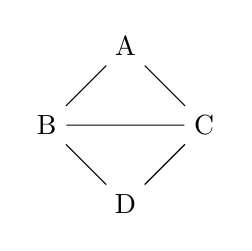
\begin{tikzpicture}
    \node (A) at (2,4) {A};
    \node (B) at (1,3) {B};
    \node (C) at (3,3) {C};
    \node (D) at (2,2) {D};

    \draw
    (A) -- (B)
    (A) -- (C)
    (B) -- (C)
    (B) -- (D)
    (C) -- (D);
    \end{tikzpicture}
    \caption{Physical topology}
    \end{subfigure}
    ~
    \begin{subfigure}[b]{0.4\textwidth}
    \begin{tikzpicture}
    \node (root) at (2,4) {A};
    \node (B) at (1,3) {B};
    \node (C) at (3,3) {C};
    \node (D) at (2,2) {D};

    \draw
    (root) -- (B)
    (root) -- (C)
    (B) -- (D);
    \end{tikzpicture}
    \caption{Logical topology}
    \end{subfigure}
    \end{center}
    \caption{An example of how STP changes the logical network topology}
    \label{fig:stp_example}
\end{figure}

Only switches will be considered for this thesis.
Hubs, while still existent, are hardly ever used and not STP capable.
We will also refer to switches as bridges, in order to be compliant with STP nomenclature.\\

Networks where STP is utilized are usually quite large.
Additionally, changes and outages are hidden by STP and redundant links in the network.
This can make it hard to keep track of the current network layout.
Debugging STP configurations is also a difficult and time consuming task.
It is possible to check STP configurations via the Simple Network Management Protocol (SNMP).
However, this requires an administrator to connect to every single bridge and jot down the STP information on their own.
While there are tools to automate this, they rely primarily on SNMP, which may not be supported by all bridges in the network.\\

The aim of this project was to create a versatile tool for STP visualization.
This tool had the following requirements:
\begin{itemize}
    \item \textbf{STP only}: the tool could only rely on STP packets
    \item \textbf{Low traffic}: the tool should create as low a traffic as possible
    \item \textbf{Passive}: the tool could not provoke any changes in the network and only use packets obtained passively
    \item \textbf{Distributed}: the tool is to be run on multiple nodes, to send information to a central server where everything is pieced together
    \item \textbf{Low hardware load}: the tool must run on simplistic hardware (e.g. a Raspberry Pi) or on a regular PC without slowing it down noticeably
    \item \textbf{No maintenance}: once set up, the tool must not require any maintenance (except when updating to a new version)
\end{itemize}

We decided to write the tool in C++.
%TODO: finish implementation idea
